
\documentclass[review]{elsarticle}

\usepackage{lineno,hyperref}
\usepackage{amsmath}
\usepackage{amsfonts}
\usepackage{amssymb}

\modulolinenumbers[5]

%\journal{Journal of \LaTeX\ Templates}

%%%%%%%%%%%%%%%%%%%%%%%
%% Elsevier bibliography styles
%%%%%%%%%%%%%%%%%%%%%%%
%% To change the style, put a % in front of the second line of the current style and
%% remove the % from the second line of the style you would like to use.
%%%%%%%%%%%%%%%%%%%%%%%

%% Numbered
%\bibliographystyle{model1-num-names}

%% Numbered without titles
%\bibliographystyle{model1a-num-names}

%% Harvard
%\bibliographystyle{model2-names.bst}\biboptions{authoryear}

%% Vancouver numbered
%\usepackage{numcompress}\bibliographystyle{model3-num-names}

%% Vancouver name/year
%\usepackage{numcompress}\bibliographystyle{model4-names}\biboptions{authoryear}

%% APA style
%\bibliographystyle{model5-names}\biboptions{authoryear}

%% AMA style
%\usepackage{numcompress}\bibliographystyle{model6-num-names}

%% `Elsevier LaTeX' style
\bibliographystyle{elsarticle-num}
%%%%%%%%%%%%%%%%%%%%%%%

\begin{document}

\begin{frontmatter}

\title{Gaokerena: A Small Persian Medical Language Model Family}


\author[ui]{Mehrdad Ghassabi\corref{mycorrespondingauthor}}
\ead{m.ghassabi@eng.ui.ac.ir}

\author[ui]{Hamidreza Baradaran Kashani} 
\author[ut]{Pedram Rostami}
\author[uw]{Sadra Hakim}
\author[au]{Zahra Kazemi}
\author[iums]{Amirhossein Poursina}
\author[ui]{Milad Tavakoli}
\author[utd]{Audrina Ebrahimi}

\address[ui]{University of Isfahan, Isfahan, Iran}
\address[ut]{University of Tehran, Tehran, Iran}
\address[uw]{University of Windsor, Windsor, ON, Canada}
\address[au]{Alzahra University, Tehran, Iran}
\address[iums]{Isfahan University of Medical Sciences, Isfahan, Iran} 
\address[utd]{University of Texas at Dallas, Dallas, TX, USA}

\cortext[mycorrespondingauthor]{Corresponding author}
\begin{abstract}
The integration of artificial intelligence into medical question-answering systems has advanced rapidly; however, research remains predominantly focused on English, leaving low-resource languages like Persian significantly underserved. To address this gap, this paper introduces Gaokerena, a novel family of compact Persian medical language models optimized for deployment on consumer-grade hardware. As a foundational step toward localized digital healthcare, we first present Gaokerena-V, developed by training a baseline model on a newly curated 90-million-token Persian medical corpus and 20,000 expert-vetted physician Q\&A pairs, which improved performance on a translated medical MMLU benchmark from 46.28\% to 49.31\%. Second, recognizing the critical demands of clinical reasoning, we developed Gaokerena-R by integrating a Chain-of-Thought approach with two novel Reinforcement Learning with AI Feedback (RLAIF) frameworks to optimize preference-based reasoning. Despite utilizing the same baseline architecture and a smaller dataset than Gaokerena-V~\cite{b1}, Gaokerena-R~\cite{b2} achieved a superior benchmark score of 52.98\%. Furthermore, both models are equipped with custom-developed uncertainty heads that predict the model’s confidence in its responses based solely on internal hidden states. While these results demonstrate significant progress in Persian medical language modeling and proactive safety estimation, current performance levels remain insufficient for direct clinical application, highlighting the necessity for further research into robust knowledge acquisition and rigorous safety verification prior to real-world deployment.
\end{abstract}

\begin{keyword}
small medical language model \sep low resource languages  \sep reasoning language models \sep reinforcement learning with ai feedback

\end{keyword}

\end{frontmatter}

%\linenumbers

\section{Introduction}

The advent of the transformer architecture, introduced in the seminal work ``Attention is All You Need''~\cite{b3}, has catalyzed a rapid evolution in the field of natural language processing (NLP). This architectural breakthrough has enabled the development of increasingly sophisticated Large Language Models (LLMs) that leverage self-attention mechanisms to comprehend and generate human language with unprecedented accuracy. Consequently, the integration of artificial intelligence (AI) has surged across various high-stakes domains. This is particularly evident in the medical field, where AI-driven solutions are actively deployed to enhance diagnostic precision, optimize patient care, and streamline administrative workflows.

Modern language models span a vast spectrum of scales, ranging from lightweight models with a few billion parameters to massive architectures exceeding trillions of parameters. While ultra-large models exhibit remarkable general knowledge and highly accurate reasoning, their immense computational requirements preclude deployment on consumer-grade, local hardware. In clinical and medical contexts, this operational bottleneck introduces significant privacy and data security concerns, as sensitive patient information must often be transmitted to external cloud servers. Accordingly, there is a critical and growing imperative for specialized, small medical language models capable of local execution on edge devices to ensure strict data confidentiality.

Despite the extensive research and development dedicated to English-centric small medical language models, such as Medreason~\cite{b4}, a profound disparity remains regarding the resources available for non-English languages. This resource scarcity is highly pronounced for the Persian language; despite its large, global community of speakers, the complete absence of a high-performing, localized small medical language model leaves a critical gap in clinical AI accessibility. To the best of our knowledge, at the beginning of this research, the only existing Persian medical language model was Sina-BERT~\cite{b5}, which is a closed-source solution with respect to both weights and training data. Furthermore, Sina-BERT is restricted to a non-generative encoder architecture, severely limiting its adaptability for conversational clinical tasks. This lack of open-source, generative alternatives severely hinders reproducibility and slows down the integration of AI solutions within the Persian-speaking medical community.

Beyond the absence of localized, small medical language models, the Persian medical NLP landscape suffers acutely from data scarcity; paradoxically, this gap stems from the underutilization of existing digital assets rather than a fundamental lack of raw source material. Active Persian-language medical forums (e.g., Drhast, Doctor-yab) and authoritative online medical magazines (e.g., Hidocor, Niniban) host vast repositories of expert-curated content and authentic patient-doctor interactions that, if systematically crawled, rigorously cleaned, and properly structured, represent invaluable corpora for domain-specific language modeling. Furthermore, high-stakes medical examinations administered annually present an untapped resource for academic evaluation and fine-tuning if systematically extracted from legacy PDF formats. Complementing these localized efforts, the strategic translation of established, high-quality English medical datasets offers another vital trajectory to alleviate data scarcity and bridge the resource gap in Persian medical AI.

To address these compounding challenges, this paper introduces a comprehensive suite of data resources and open-source language models tailored specifically for the Persian medical domain. Utilizing these diverse datasets, we develop and introduce two localized small medical language models: \textbf{Gaokerena-V} and \textbf{Gaokerena-R}, the latter of which incorporates advanced reasoning capabilities. Furthermore, to validate their efficacy, we rigorously evaluate the performance of both models using our newly curated and structured benchmark datasets.
\footnote{
All research artifacts, including the curated datasets, model weights, and generated model responses, are publicly available at github.com/Mehrdadghassabi/Gaokerena-V and github.com/Mehrdadghassabi/Gaokerena-R
}
The core contributions of this work are summarized as follows:
\begin{itemize}
    \item \textbf{A 90-Million Token Medical Corpus:} A large-scale, domain-specific text corpus systematically crawled and curated from authoritative Persian medical magazines.
     \item \textbf{The MF3QA Dataset:} A novel, high-quality dataset of 24,000 authentic Persian patient-doctor interaction pairs, curated from active medical forums. Through a meticulous cleaning and filtering process, we distilled this subset from an initial pool of 184,000 raw interaction pairs to ensure clinical relevance and linguistic quality. The dataset is partitioned into 20,000 training, 2,000 development, and 2,000 testing samples.
     \item \textbf{A Consolidated Benchmarking Suite:} A 3,000-question medical MCQ benchmark comprising both official questions from the Iranian Basic Medical Science Exam (IBMSEE) and English-language medical questions expertly translated into Persian to ensure clinical accuracy and linguistic precision.
     \item \textbf{Translated Training Resources:} A curated collection of 18,000 Persian medical multiple-choice questions generated via machine translation of English-language medical sources. These are intended exclusively for training to mitigate the impact of potential translation artifacts on final evaluation metrics.
    \item \textbf{Novel Reasoning Frameworks:} The development of two distinct structural frameworks designed specifically to enhance the medical reasoning capabilities of localized language models, which directly underpinned the training of Gaokerena-R.
    \item \textbf{Localized Persian Medical Language Models:} The introduction of Gaokerena-V and Gaokerena-R, two pioneering small Persian medical language models optimized for consumer hardware; while they demonstrate robust medical knowledge retrieval, we explicitly note they are research artifacts and not yet cleared for real-world clinical deployment.
\item \textbf{Uncertainty Estimation Framework:} The design and implementation of dedicated uncertainty estimation heads for the Gaokerena models. These heads leverage the model’s internal states to quantify predictive uncertainty, enabling confidence scoring and risk mitigation during medical inference.
\end{itemize}

\section{Literature Review}

\subsection{English Small Medical Language Models}
Substantial advancements in specialized medical language models have focused heavily on extracting cognitive processes and structural reasoning. Prominent among these developments is the Meerkat model family~\cite{b6}, which introduces a framework centered on extracting medical Chain-of-Thought (CoT)~\cite{b7} reasoning trajectories directly from authoritative medical textbooks. By fine-tuning a foundational language model on these reasoning paths alongside complementary biomedical datasets, Meerkat shifts the focus from simple factual retrieval to the underlying decision-making processes inherent to clinical practice. This design allows the model to simulate expert medical reasoning, making it highly effective for complex, multi-step clinical dialogues.

Advanced reasoning has also been pursued through algorithmic search and process evaluation, as demonstrated by the MedSSS~\cite{b8} framework. To enhance medical reasoning, researchers meticulously structured the intermediate steps between a question and its final answer by utilizing the Monte Carlo Tree Search (MCTS) algorithm over multiple-choice medical question datasets to generate systematic, step-by-step reasoning paths. This process yielded three distinct synthetic datasets for training: a supervised fine-tuning dataset to train the policy model with high-quality reasoning chains; a preference dataset for Reinforcement Learning (RL) to help the model distinguish between strong and weak responses; and a soft-label dataset to train a process reward model. Ultimately, the trained policy model serves as the primary reasoning engine, while the process reward model acts as a guide during generation, continuously evaluating the logical coherence and medical accuracy of each reasoning step.

While the aforementioned models focus on enhancing reasoning capabilities, MedMobile~\cite{b9} adopts a different approach to addressing low-resource medical languages. Utilizing Microsoft’s Phi-3-mini~\cite{b10} as its baseline architecture, MedMobile was fine-tuned on a blended dataset of human-curated and synthetic medical data. This optimization enables the model to run efficiently on resource-constrained mobile devices, providing ubiquitous and privacy-preserving access to high-quality clinical guidance without the need for persistent cloud connectivity.

\subsection{Persian Small Language Models}
Although many current multilingual models include support for Persian, smaller-scale variants frequently suffer from language mixing, grammatical issues, and a lack of linguistic nuance. This limitation is driven by a severe data imbalance, as these models are trained predominantly on massive English and Chinese corpora, leaving Persian as a negligible fraction of the training data. To bridge this gap, the Cohere for AI research team introduced Aya-Expanse~\cite{b11}, a family of multilingual models featuring a specialized training paradigm. Instead of relying entirely on imbalanced, human-generated web data, Aya-Expanse utilizes high-quality synthetic data generated by larger, state-of-the-art models. While this approach grants the model a sophisticated grasp of Persian syntax and semantics, its general-purpose nature results in performance degradation within highly specialized domains, particularly regarding medical knowledge and clinical reasoning.

Another effort to address native NLP limitations, researchers at the University of Tehran developed PersianMind~\cite{b12}, an open-source bilingual model optimized for cross-lingual Persian-English tasks. Given the historical shortage of multilingual models that supported Persian when the project began, the developers expanded the tokenizer of LLaMA-2~\cite{b13} to support Persian tokens and trained the network to master the language's syntax and semantics. Yet, much like Aya-Expanse, PersianMind functions strictly as a general-purpose model. Devoid of exposure to deep, domain-specific clinical corpora during its pre-training and instruction-tuning phases, it exhibits the same constraints in advanced clinical reasoning and medical QA. Additionally, Aya-Expanse benefits from a much larger training corpus, granting it superior general knowledge. For these reasons, we ultimately chose Aya-Expanse as our baseline architecture, focusing our efforts on mitigating its specialized domain deficiencies for healthcare applications.

\section{Data Collection}
As previously noted, the Persian medical domain severely lacks both specialized small language models and high-quality datasets suitable for research. Consequently, to develop and evaluate Persian medical language models, it was essential to curate a proprietary dataset tailored to these research requirements. The data collection pipeline integrated various methodologies, including human and machine translation of existing foreign-language datasets, web scraping diverse sources, and extracting multiple-choice question (MCQ)  from PDF documents to build a comprehensive and functional corpus.

\subsection{Persian Medical Corpus}
The absence of a dedicated Persian medical corpus poses a significant challenge for researchers and developers aiming to build Persian medical models. Without the high-quality, domain-specific text data essential for training artificial intelligence models, these efforts may face major bottlenecks, ultimately hindering the development of advanced medical technologies and solutions tailored for the Persian-speaking population. To address this issue, we have compiled a comprehensive dataset comprising approximately 90 million tokens across roughly 102,000 articles, each authored by medical professionals.
\footnote{
To access this corpus, you can visit huggingface.co/datasets/gaokerena/medical\_corpus.
}

Garcia-Ferrero et al.~\cite{b14}
compiled a collection of medical texts spanning four languages (English, French, Spanish, and Italian), which can be compared to our dataset as illustrated in Table~\ref{corpus_comparison}. The corpus we have gathered was crawled from online medical journals; the specific contribution of each journal to this corpus is displayed in Figure~\ref{fig1}.

\begin{figure}[htbp]
		\centerline{
\includegraphics[width=0.5\textwidth]{fig1.png}}
		\caption{Medical corpus sources}
		\label{fig1}
\end{figure}

\begin{table}[ht]
		\centering
		\begin{tabular}{|l|c|c|}  % Using vertical lines for a simple table
			\hline
			language& no. tokens & collected by \\ \hline
			English & 1.1B & I. Garcia Ferrero et al. \\ \hline
			Spanish & 950M & I. Garcia Ferrero et al.  \\ \hline
			French & 675M & I. Garcia Ferrero et al.  \\ \hline
			Italian& 143M &  I. Garcia Ferrero et al.  \\ \hline
			Persian& 90M & us	\\ \hline
		\end{tabular}
                   \caption{Comparison of Our Corpus with Corpora Collected by I. Garcia Ferrero et al.}
		\label{corpus_comparison}
\end{table}

\subsection{MF3QA}
The collection of a real-world doctor-patient question-answering (QA) dataset is crucial for enhancing the capabilities of large language models (LLMs) in the healthcare domain. Despite the existence of reputable online medical forums like Drhast, the Persian language lacked a comprehensive dataset of this nature at the onset of this research; therefore, we have introduced the first Medical Free-Form Farsi Question Answering dataset (MF3QA).
\footnote{
To access this dataset, you can visit huggingface.co/datasets/gaokerena/MF3QA.
}

Such a dataset allows models to learn valuable information derived from authentic interactions between healthcare providers and patients. By analyzing these real-world exchanges, language models can grasp the nuances of medical terminology, patient concerns, and the context surrounding healthcare inquiries. Furthermore, this dataset equips models with the ability to learn not just the factual content of responses but also the appropriate structure and tone for professional communication. This dual learning process is essential, as it enables the model to generate accurate, empathetic, and contextually relevant responses, ultimately improving patient communication and support in medical environments. In this context, Yang Liu~\cite{b15} highlights several real-world doctor-patient question-answering datasets in his survey; a comparison of these datasets with ours is provided in Table~\ref{mf3qa_comparison}.

\begin{table}[ht]
    \centering
    \begin{tabular}{|l|c|c|}  
        \hline
        \textbf{Dataset Name} & \textbf{Language} & \textbf{No. Records}  \\ \hline
        ChatDoctor~\cite{b16} & English & 100K \\ \hline
        CMtMedQA~\cite{b17} & Chinese & 68K  \\ \hline
        DISC-Med-SFT~\cite{b18} & Chinese & 465K \\ \hline
        HuatuoGPT-sft-data-v1~\cite{b19} & Chinese & 226K  \\ \hline
        Huatuo-26M~\cite{b20} & Chinese & 26M  \\ \hline
        MedDialog~\cite{b21} & Chinese \& English & 3.66M  \\ \hline
        Medical-Meadow~\cite{b22} & English & 160K  \\ \hline
        MF3QA & Persian & 24K\\ \hline
    \end{tabular}
    \caption{Comparison of our dataset with existing medical QA datasets}
    \label{mf3qa_comparison}
\end{table}

To construct our dataset, we initially crawled more than 180,000 raw question-answer (QA) pairs from prominent Persian medical forums; the individual contributions of each forum are illustrated in Figure~\ref{fig2}. We subsequently implemented a rigorous hybrid pipeline combining automated filtering with manual verification. Our data curation methodology draws inspiration from the approach introduced by Li et al.~\cite{b16} for the ChatDoctor model, in which approximately half of the scraped English QA pairs were discarded based on answer length, as truncated responses can inhibit a Large Language Model’s (LLM) capacity to generate comprehensive explanations.

However, we encountered a significantly more pronounced data-filtering bottleneck: Persian medical practitioners online tend to provide much more concise responses than their English-speaking counterparts. Consequently, to maintain high training quality and clinical relevance, we filtered out over 80\% of our raw records. Furthermore, our preprocessing pipeline employed a more sophisticated multi-stage strategy than the simple length thresholds utilized in ChatDoctor. First, to shift the token-count distribution toward longer, more informative responses, we applied a randomized omission strategy for answers containing fewer than 50 tokens within the training and development sets. To preserve the integrity of our evaluation metrics, this random exclusion was not applied to the test split; instead, we manually reviewed every QA pair in the test set to verify factual accuracy and clinical validity. For the test set specifically, we extracted data from the Doctor-yab and Isovisit platforms and ensured linguistic diversity by translating the K-QA question-answering dataset~\cite{b23} and appending it to our test split. Additionally, every record underwent intensive manual review to eliminate spam, duplicates, and low-quality entries. This rigorous process yielded a final dataset consisting of 20,000 QA pairs for the training set, 2,000 for the development set, and 2,000 for the test set.

It is important to note that the Drhast platform does not provide all doctor-patient interaction records directly; it only offers public access to the 2,000 most recent dynamic records. Furthermore, each record is linked to approximately 100 related entries, significantly complicating the crawling process. To address this challenge, we modeled the data as a graph and performed a Breadth-First Search (BFS) traversal. The BFS execution utilized an iterative loop, selecting available records from the initial 2,000 as root nodes to explore their linked neighbors. By repeatedly performing BFS with new roots, we ensured broader coverage of the dataset while preventing redundancy through post-iteration duplicate filtering. Because the Drhast records are dynamic and change as new questions are posted, we were able to utilize newly added records as roots for subsequent BFS runs. This iterative process successfully extracted 120,000 records out of an estimated 200,000 within a two-week period.
\begin{figure}[htbp]
    \centerline{
\includegraphics[width=1.0\textwidth]{fig2.png}}
    \caption{MF3QA sources}
    \label{fig2}
\end{figure}


\subsection{Persian Medical Multiple Choice Question Dataset}
While free-form question-answering (QA) datasets are invaluable, the inclusion of multiple-choice question (MCQ) datasets is equally critical for the development of robust medical language models. Various training paradigms, such as those utilized for introducing the MedSSS medical language model~\cite{b8}, specifically require high-quality MCQ datasets to facilitate specialized instruction tuning. Furthermore, evaluating a medical language model using a standardized MCQ test set remains the gold standard for measuring clinical reasoning, as it provides an objective, quantifiable metric for assessing a model’s diagnostic and pharmacological knowledge.

To establish a rigorous benchmark for Persian medical language models, we curated two distinct, high-precision test sets:
firstly We have extracted approximately 2,000 questions from the Iranian Basic Medical Science Entrance Exams (2021–2024). These questions were meticulously converted from PDF formats into a structured digital format to serve as a domain-specific, localized benchmark.
\footnote{
To access this dataset, you can visit huggingface.co/datasets/gaokerena/KOPP.
}
secondly We performed a meticulous manual translation of the medical portion of the Massive Multitask Language Understanding (MMLU) dataset~\cite{b24}, comprising approximately 1,000 questions. This allows for standardized cross-lingual comparison with global benchmarks.
\footnote{
To access this dataset, you can visit huggingface.co/datasets/gaokerena/FA\_MED\_MMLU.
}

Recognizing that training data is less sensitive to minor semantic variations than evaluation data, we employed a scalable machine translation framework to develop a large-scale training corpus. Given the absence of a comprehensive Persian medical MCQ dataset at the time of this research, we utilized the cost-efficient yet highly capable DeepSeek-V3 model~\cite{b25} to translate a significant portion of the MedMCQA dataset~\cite{b26} from English to Persian.
\footnote{
To access this dataset, you can visit github.com/Mehrdadghassabi/Gaokerena-R/tree/main/dataset/medmcqa\_translation\_filterd.
}

To ensure thematic diversity, questions were sampled randomly from the MedMCQA pool, ensuring broad coverage of medical disciplines, including physiology, pharmacology, pathology, and clinical practice. To maintain high data quality, we implemented a dual-referee validation process using two independent models: Grok-3-mini~\cite{b27} and GPT-4.1-mini~\cite{b28}. Each referee was tasked with evaluating the translated questions and their corresponding options for semantic accuracy, linguistic fluency, and the preservation of specialized medical terminology. A translation was only accepted into our final dataset if both referees independently assigned it a perfect score of five out of five. Through this rigorous, multi-stage process, we successfully curated a high-quality dataset consisting of approximately 18,000 medically accurate, Persian-language multiple-choice questions.

\section{Gaokerena Models}
We introduce two lightweight Persian medical language models, Gaokerena-V and Gaokerena-R, both utilizing Aya-Expanse-8B as their foundational architecture. The former, Gaokerena-V, is developed via domain adaptation, trained on a strategically selected subset of our curated medical corpus in conjunction with the MF3QA dataset to optimize for medical proficiency and efficiency. The latter, Gaokerena-R, is designed to enhance logical reasoning through specialized post-training on Multiple-Choice Questions (MCQs). By utilizing our proposed framework to distill reasoning from a larger teacher model, Gaokerena-R is specifically optimized for medical reasoning.

\subsection{Gaokerena-V}
To effectively adapt the 8-billion-parameter \textit{Aya-Expanse} checkpoint to the nuances of the Persian medical domain, we adopted a structured two-stage fine-tuning strategy consisting of a domain-adaptation stage and an instruction-tuning stage. This two-stage paradigm establishes a coherent training pipeline: the initial stage facilitates the internalization of dense medical knowledge and factual information, providing a robust foundation for the subsequent stage, which focuses on refining instruction-following capabilities and the communication protocols required for effective medical QA. Across both stages, the baseline model was trained on a total of 60 million new tokens. A comprehensive summary of the hyperparameters utilized for both stages is provided in Table~\ref{ft_it_training_details}.

During the domain-adaptation stage, we performed domain-adaptive pre-training on 60\% of our curated medical corpus. This phase was designed to immerse the model in specialized Persian medical terminology, linguistic structures, and foundational clinical concepts. To ensure computational efficiency and mitigate the risk of catastrophic forgetting of the model’s general-purpose capabilities, we employed Low-Rank Adaptation (LoRA)~\cite{b29}. By injecting trainable rank-decomposition matrices into the self-attention layers, we captured domain-specific nuances without requiring a full-parameter update. The steady convergence of the training process, reflecting the successful internalization of the medical corpus, is illustrated by the decreasing loss trajectory in Figure~\ref{fig3}.

In the subsequent instruction-tuning stage, we transitioned to specialized tuning aimed at refining the model’s conversational fluency. We utilized the full training split of our newly constructed MF3QA dataset, which comprises high-quality, real-world doctor-patient interactions. To further optimize the model for task-specific performance specifically the interpretation of symptoms and the provision of contextually relevant medical guidance we continued using the LoRA framework. To prevent overfitting during this stage, we employed more conservative hyperparameters, specifically utilizing a lower LoRA rank and alpha, alongside an increased LoRA dropout rate. The loss trajectory for this instruction-tuning phase is illustrated in Figure~\ref{fig4}.
\begin{table}[ht]
		\centering
		\begin{tabular}{|l|c|c|}  
			\hline
			& Domain-adaptation & Instruction-tuning \\ \hline
			on & medical\_corpus & MF3QA \\ \hline
			Number of epochs & 1& 1\\ \hline
			Batch size & 2 &  2 \\ \hline
			Number of gradient &  &  \\ 
                        accumulation steps &16  &16 \\ \hline
                        Optimizer & AdamW & AdamW\\ \hline
                        Learning rate &5E-4 & 5E-4 \\ \hline
			Maximum gradient norm& 0.3 & 0.3 \\ \hline
			Warmup ratio&0.03 &0.03	\\ \hline
                        Weight decay rate & 0.1  &0.5	\\ \hline
                        Maximum context length & 1024  &1024	\\ \hline
                        Padding strategy & left side padding   & left side padding	\\ \hline
                        Lora rank &8   &2	\\ \hline
                        Lora alpha &16   &2	\\ \hline
                        Lora dropout rate &0.05   &0.4	\\ \hline
                        Target modules &all linear layers   &all linear layers	\\ \hline
		\end{tabular}
                   \caption{Gaokerena-V Training Hyperparameters}
\label{ft_it_training_details} 
\end{table}

\begin{figure}[h]
    \centering
    
\includegraphics[width=1.0\linewidth]{fig3.png}
    \caption{fine-tuning loss curve}
    \label{fig3}
\end{figure}

\begin{figure}[h]
    \centering
    
\includegraphics[width=1.0\linewidth]{fig4.png}
    \caption{instruction-tuning loss curve}
    \label{fig4}
\end{figure}

\subsection{Gaokerena-R}
To introduce \textbf{Gaokerena-R}, which enhances the reasoning capabilities of the Aya-expanse-8b baseline, we propose a two-pronged Reinforcement Learning from AI Feedback (RLAIF)~\cite{b30} pipeline. Our objective is to transform the base model into a specialized medical reasoning agent by constructing a high-quality preference dataset $\mathcal{D}=\{(x,y_w,y_l)\}$, where $x$ denotes a medical question, $y_w$ is a preferred reasoning trajectory, and $y_l$ is a rejected response. We then optimize the student policy $\pi_\theta$ using Direct Preference Optimization (DPO)~\cite{b31} to align it with these high-quality trajectories. The optimization objective is defined by the DPO loss in Formula~\ref{fr:DPOloss}, and its convergence is illustrated by the DPO loss curve shown in Figure~\ref{fig5}.

To enhance the medical reasoning capabilities of the student policy $\pi_\theta$, we employ a teacher--student architecture where the student ($\pi_S$) is the baseline \texttt{Aya-Expanse-8b} model and the teacher ($\pi_T$) is a high-capacity reasoning model (DeepSeek-R~\cite{b32}). We generate preference pairs using two complementary strategies to provide diverse training signals; these signals allow the student to learn medical reasoning behaviors from the teacher.

The first strategy, \textit{Expert-Guided Synthesis}, contrasts the baseline model's flawed logic with expert-level reasoning. For a given question $x$, the student model $\pi_S$ produces an initial response $y_{\text{init}}$. If $y_{\text{init}}$ is deemed incorrect, it is assigned as the rejected response ($y_l$). To obtain the preferred trajectory ($y_w$), the teacher model $\pi_T$ is prompted with the ground-truth answer and instructed to generate a detailed, correct Chain-of-Thought (CoT) explanation. This yields a preference triple $(x,y_w,y_l)$ that explicitly separates erroneous student reasoning from verified expert trajectories, as illustrated in Figure~\ref{fig6}.

The second strategy, \textit{Iterative Self-Correction}, encourages intrinsic error correction within the student's own distribution via an iterative feedback loop. To remain computationally efficient while maximizing the utility of each sample, we use a critique-based refinement process. If $y_{\text{init}}$ is incorrect, the teacher $\pi_T$ generates a textual critique $c$ that highlights the conceptual error without revealing the correct solution. The student is then prompted with this critique to produce a corrected response $y_{\text{retry}}$. If $y_{\text{retry}}$ is correct, it becomes the preferred response ($y_w$), while the original incorrect response $y_{\text{init}}$ serves as the rejected response ($y_l$). This design grounds preferred trajectories in the student's latent space, promoting more stable convergence. The overall workflow is depicted in Figure~\ref{fig7}.

During data synthesis, we find that \textit{Expert-Guided Synthesis} is the dominant contributor to the preference dataset construction; for every 19 preference pairs generated by this strategy, typically only one pair is successfully synthesized through \textit{Iterative Self-Correction}. This hybrid scheme balances expert-led guidance with autonomous student correction. The final preference dataset contains approximately $11{,}000$ pairs, totaling roughly $2$ million preferred tokens and $2.5$ million rejected tokens.

\begin{equation}
\begin{aligned}
    \mathcal{L}_{\text{DPO}} =
    -\mathbb{E}_{(x,y_w,y_l)\sim \mathcal{D}}
    \left[
        \log \sigma \left(
            \beta \log \frac{\pi_{\theta}(y_w\mid x)}{\pi_{\text{ref}}(y_w\mid x)}
            - \beta \log \frac{\pi_{\theta}(y_l\mid x)}{\pi_{\text{ref}}(y_l\mid x)}
        \right)
    \right]
\end{aligned}
\label{fr:DPOloss}
\end{equation}

where $\sigma$ denotes the sigmoid function and $\beta$ controls the strength of the update relative to the reference model. Minimizing $\mathcal{L}_{\text{DPO}}$ implicitly increases the probability of valid reasoning trajectories ($y_w$) while suppressing flawed logic ($y_l$), thereby distilling the teacher's reasoning into the Gaokerena-R model.



\begin{figure}[h]
    \centering
    
\includegraphics[width=1.0\linewidth]{fig5.png}
    \caption{DPO loss curve}
    \label{fig5}
\end{figure}

\begin{figure}[h]
    \centering
    
\includegraphics[width=1.0\linewidth]{fig6.png}
    \caption{Method 1 Block Diagram}
    \label{fig6}
\end{figure}

\begin{figure}[h]
    \centering
    
\includegraphics[width=1.0\linewidth]{fig7.png}
    \caption{Method 2 Block Diagram}
    \label{fig7}
\end{figure}

\section{Uncertainty Heads}
\label{sec:uhead}
Our methodology builds upon the LLM Uncertainty Head (LUH) framework introduced by Shelmanov et al~\cite{b33}, which augments a pretrained language model with a lightweight auxiliary head that detects hallucinated claims during generation. The head reads the frozen backbone's internal signals---per-layer attention maps and token probability statistics---and predicts, for each extracted claim, whether it is factually supported or fabricated. Because the backbone remains frozen and only the head is optimised, the approach adds negligible parameter overhead, requires no external retrieval, and needs no repeated sampling at inference time. This last property is what distinguishes it from the consistency-based estimates used elsewhere in this work: a single forward pass yields a calibrated per-claim signal.

In its original implementation for Mistral-7B~\cite{b34} on English data, the pipeline extracts atomic, verifiable claims from generated responses, aligns each claim with its exact token span, and trains the head with ternary token labels: $1$ for tokens belonging to hallucinated claims, $0$ for tokens belonging to supported claims, and $-100$ to mask every non-claim token (stopwords, punctuation, section headings) so that it contributes nothing to the loss. This ensures the head learns exclusively from semantically meaningful content, which is critical for accurate uncertainty estimation.

\subsection{Motivation: Response Instability in Aya-Expanse and its Derivatives}
Before training an uncertainty head, it is worth establishing that the Aya-Expanse family exhibits measurable output instability, and that this instability is not removed---and can even be amplified---by domain adaptation.

We conducted a simple experiment in which Aya-Expanse-8B, Gaokerena-V, and Med-Gemma each answered the September 2023 Iranian Basic Medical Sciences Entrance Examination (IBMSEE)\footnote{Available at \texttt{huggingface.co/datasets/gaokerena/KOPP}}. Every model was run five times over the identical question set under Chain-of-Thought prompting~\cite{b7}\footnote{We use Chain-of-Thought prompting because it unveils uncertainty more clearly than direct prompting.}. We then measured, per model, the number of questions for which all five runs selected a single option, the number for which the five runs collectively covered every available option, and the predictive entropy over the option distribution. Results are reported in Table~\ref{tab:uhead_consistency}.

Med-Gemma selected the same option in all 168 questions, yielding zero entropy: its answers are fully determined. The two Aya-derived models behaved very differently, agreeing across all five runs on only 44 and 10 questions respectively. The comparison between Aya-Expanse-8B and Gaokerena-V is the more consequential one. Although Gaokerena-V acquires substantially more Persian medical knowledge by continued training on 57M Persian medical tokens---and scores 4.17 percentage points higher in accuracy---it becomes \emph{more} uncertain than the baseline it was derived from, with entropy rising from 1.21 to 1.62 and the number of fully consistent questions falling from 44 to 10. Domain adaptation of this backbone therefore buys knowledge at the cost of stability, which is a warning about the vulnerability of Aya-Expanse to continued pretraining and the attendant risk of hallucination.

One plausible explanation lies in how Aya-Expanse was trained. Its pipeline combines fine-tuning on synthetic data, iterative preference training, and model merging~\cite{b35}, with synthetic data generated by a variety of teacher models. Each teacher contributes its own perspectives and biases, producing a rich but internally inconsistent training distribution; the amalgamation of these differing signals may surface later as instability in the student's outputs.

This finding motivates the remainder of this section. Because sampling-based consistency is both expensive---it requires five generations per question---and, as Table~\ref{tab:uhead_consistency} shows, a coarse instrument, we instead train a dedicated uncertainty estimator that produces a per-claim reliability signal from a single forward pass.

\begin{table}[ht]
\centering
\begin{tabular}{|l|c|c|c|}
\hline
\textbf{} & \textbf{Gaokerena-V} & \textbf{Aya-Expanse} & \textbf{Med-Gemma} \\ \hline
Accuracy & \textbf{38.69} & 34.52 & 37.50 \\ \hline
Number of & & & \\
single option taken & 10 & 44 & \textbf{168} \\ \hline
Number of & & & \\
all options taken & 10 & 7 & \textbf{0} \\ \hline
Entropy & 1.62 & 1.21 & \textbf{0} \\ \hline
Prompt & CoT & CoT & CoT \\ \hline
Number of & & & \\
parameters & 8 billion & 8 billion & 4 billion \\ \hline
\end{tabular}
\caption{Comparison of model consistency on IBMSEE (September 2023), five runs per question.}
\label{tab:uhead_consistency}
\end{table}

\subsection{Persian Claim-Level Dataset Construction}
Transferring LUH to Persian is not a matter of retraining the head on translated data. Persian is written in a right-to-left script and is richly inflected, which complicates substring matching and span extraction, and the Aya-Expanse tokenizer segments Persian with a subword vocabulary in which a single English claim token may map to several Persian tokens. An earlier prototype of this work translated the original English LUH dataset into Persian and then re-established sentence- and claim-level alignment, but every translation step introduces semantic drift and every realignment step introduces ambiguity, both of which propagate directly into the token-level labels.

We therefore construct the dataset natively in Persian, so that no translation or realignment is required at any stage. The pipeline proceeds as follows.

\begin{enumerate}
\item \textbf{Question curation.} We curate a set of 1{,}600 Persian medical questions\footnote{Drawn from \texttt{huggingface.co/datasets/gaokerena/fa\_luh\_aya}} under three constraints, applied by a fully deterministic procedure with no random sampling, so that the resulting set is reproducible. At most one question is kept per base medical entity, so that the set is not dominated by near-duplicate entries. Synthetic entity variants are capped at approximately 6\% of the set, so that the head learns to detect genuine hallucination rather than an artifact of the question template. And questions are taken at even intervals across an alphabetically ordered pool of medical entities, preserving topical coverage from A to Z.

\item \textbf{Response generation.} Gaokerena-V and Gaokerena-R each answer all 1{,}600 questions with deterministic (greedy) decoding. Both models see the identical question set in the identical order, so the two resulting datasets are paired: any difference between the two trained heads is attributable to the backbone, not to which questions it was asked.

\item \textbf{Claim extraction.} Atomic, verifiable claims are extracted from each response using Persian-language prompts, so the claims are produced directly in Persian and never pass through English. Sentences shorter than 40 characters after markup is stripped are section headings and labels rather than factual assertions; these are discarded before extraction, which removes a systematic source of unverifiable claims.

\item \textbf{Claim verification.} Each extracted claim is independently fact-checked by DeepSeek-V4-Flash~\cite{b36} acting as an automatic annotator, which labels it as supported, hallucinated, or undecided. Undecided claims are retained in the released data but excluded from the loss.

\item \textbf{Token-level alignment.} Each claim is mapped to its precise token span in the Aya-Expanse tokenization of the response, explicitly accounting for subword splits. Tokens within a claim span receive that claim's binary label and all remaining tokens are masked with $-100$.
\end{enumerate}

Table~\ref{tab:uhead_datasets} reports the resulting statistics. The two datasets are closely comparable in size and class balance, with hallucination rates of 17.73\% and 18.03\%, which is what the paired design requires. Both are released publicly.\footnote{Available at \texttt{huggingface.co/datasets/gaokerena/LUH\_Gaokerena\_V} and \texttt{.../LUH\_Gaokerena\_R}} Each is divided into training, validation, and test splits of 1{,}458, 92, and 50 rows; because the underlying pool is ordered alphabetically by medical entity, the splits are drawn at even intervals across the whole range rather than as contiguous blocks, so all three cover the full topical range.

\begin{table}[ht]
\centering
\begin{tabular}{|l|c|c|}
\hline
\textbf{} & \textbf{LUH-Gaokerena-V} & \textbf{LUH-Gaokerena-R} \\ \hline
Annotated responses & 1{,}600 & 1{,}600 \\ \hline
Extracted claims & 60{,}434 & 54{,}209 \\ \hline
Supported claims & 48{,}991 & 43{,}305 \\ \hline
Hallucinated claims & 10{,}557 & 9{,}528 \\ \hline
Undecided claims & 886 & 1{,}376 \\ \hline
Hallucination rate & 17.73\% & 18.03\% \\ \hline
Supervised tokens & 61.4\% & 54.9\% \\ \hline
Positive class weight & 4.64 & 4.53 \\ \hline
\end{tabular}
\caption{Claim-level statistics of the two Persian uncertainty datasets.}
\label{tab:uhead_datasets}
\end{table}

\subsection{Head Architecture and Training}
We train a claim-level head, which pools the token representations belonging to each claim and emits one prediction per claim, rather than a token-level head. This matches the granularity at which our annotations are defined and at which a downstream user would act.

The head receives two families of features extracted from the frozen backbone: per-layer attention maps, taken from all layers with an attention history of three preceding positions, and the top-4 token probabilities at each position. On top of these it applies a two-layer transformer encoder with a hidden dimension of 768, eight attention heads, and dropout of 0.1. Only these parameters are updated; every backbone parameter is frozen, which preserves the model's generative behaviour exactly.

Because Gaokerena-V and Gaokerena-R are distributed as LoRA adapters rather than standalone checkpoints, and the LUH training path loads its backbone with a plain model constructor that has no adapter handling, we merge each adapter into the Aya-Expanse-8B base once and train the head against the resulting merged model.

The objective is a binary cross-entropy loss computed only over labelled claims. Since supported claims outnumber hallucinated ones by roughly four to one, the positive class is reweighted by the measured supported-to-hallucinated ratio of the respective training split, 4.64 for Gaokerena-V and 4.53 for Gaokerena-R. Remaining hyperparameters are listed in Table~\ref{tab:uhead_training}. Model selection is performed on the 92-row validation split using PR-AUC, with early stopping after three epochs without improvement; the 50-row test split is held out entirely and used only once, for the final score reported in Section~\ref{sec:results}. We report accuracy, precision, recall, F1, ROC-AUC, and PR-AUC.

\begin{table}[ht]
\centering
\begin{tabular}{|l|c|}
\hline
Number of epochs & 10 \\ \hline
Learning rate & 0.0001 \\ \hline
Warmup ratio & 0.05 \\ \hline
Weight decay & 0.1 \\ \hline
Batch size & 8 \\ \hline
Maximum gradient norm & 1 \\ \hline
Uncertainty & \\
head dimension & 768 \\ \hline
Uncertainty & \\
head layers & 2 \\ \hline
Uncertainty & \\
heads & 8 \\ \hline
Uncertainty & \\
head dropout & 0.1 \\ \hline
\end{tabular}
\caption{Uncertainty head training hyperparameters.}
\label{tab:uhead_training}
\end{table}

\section{Results}
\label{sec:results}
As previously discussed, multilingual Small Language Models (SLMs) often struggle with underrepresented languages, including Persian. Cohere For AI addressed this challenge by introducing Aya Expanse, which demonstrates significant improvements in Persian fluency and linguistic comprehension. However, the curse of multilinguality persists, often resulting in performance trade-offs. In this research, we aim to mitigate these limitations by exploring various methods to enhance medical reasoning capabilities within the Persian context. Consequently, this section presents a comprehensive evaluation of our proposed models, benchmarking their performance against established alternatives to assess their effectiveness in specialized medical tasks.

\subsection{Gaokerena-V Results}
Given the scarcity of publicly available, specialized Persian medical Small Language Models (SLMs), we benchmarked the Gaokerena-V model against several general-purpose alternatives, including its baseline (Aya-Expanse-8B), PersianMind, and Qwen2.5~\cite{b37}.

As presented in Table \ref{tab:model_results_vs_general_purpose_languages}, Gaokerena-V achieved a significant milestone by surpassing the 36\% passing threshold of the Iranian Basic Medical Sciences Entrance Exam. To our knowledge, this makes it the first Persian-language model under 8 billion parameters to successfully pass this examination. Furthermore, Gaokerena-V demonstrated superior performance on the translated MMLU dataset, consistently outperforming other models across most sub-categories, thereby validating its efficacy in medical knowledge synthesis and generation in Persian.

Notably, the model achieved a 7.4\% improvement in the anatomy category over the baseline. We attribute this gain to the relative abundance of anatomy-focused material in reputable Persian digital publications. Conversely, the more moderate gains in other sub-categories highlight a critical bottleneck: the lack of comprehensive, high-quality medical corpora in Persian, which restricts further performance optimization.

Finally, Table \ref{tab:model_results_vs_general_purpose_languages} reveals that while PersianMind exhibits low inference latency, this is primarily an artifact of its tendency to produce truncated, overly concise responses. In several categories, PersianMind’s performance proved negligible, effectively mirroring the scores of random chance, which underscores its limitations in complex medical reasoning tasks.

	\begin{table}[ht]
		\centering
		\begin{tabular}{|l|c|c|c|c|}  % Using vertical lines for a simple table
			\hline
			\textbf{} & \textbf{gao} & \textbf{Aya-} &  &  \\ 
			& \textbf{kerena-V} & \textbf{Expanse-8b} & \textbf{Qwen} & \textbf{Persian} \\
			& (ours) & (baseline) & \textbf{2.5} & \textbf{Mind} \\ \hline
			MMLU-anatomy(fa)  & \textbf{48.14} & 40.74 & 41.48 & 25.18 \\ \hline
			MMLU- & \textbf{53.0} & 49.0 & 52.0 & 34.0 \\ 
                            medical-genetics(fa)&  &  &  &  \\ \hline
			MMLU- & 43.93 & \textbf{44.51} & 43.35 & 20.23 \\ 
                            college-medicine(fa)&  &  &  &  \\ \hline
			MMLU-& \textbf{55.47} & 52.07 & 47.92 & 25.28 \\
			clinical-knowledge(fa)&  &  &  &  \\ \hline
			MMLU-& \textbf{47.05} & 45.58 & 43.01 & 23.89 \\ 
			professional-medicine(fa)&  &  &  &  \\ \hline
			MMLU-college-biology(fa)& \textbf{47.22} & 45.14 & 42.36 & 32.63 \\ \hline
			MMLU(avg) & \textbf{49.31} & 46.64 & 45.17 & 25.89 \\ \hline
			IBMSEE Sept2023 & \textbf{38.69} & 34.52 & 33.33 & 19.64 \\  \hline
			Number of parameters & 8b & 8b & 7.6b & 6.8b \\ \hline
			Inference time & $\approx 10s$ & $\approx 10s$ & $\approx 15s$ & $\approx 2s$ \\  \hline

		\end{tabular}
                   \caption{
			Gaokerena-V Performance Comparison with Other models
		}
		\label{tab:model_results_vs_general_purpose_languages}
	\end{table}

\subsection{Gaokerena-R Results}
As a medical-reasoning-enhanced version of Aya-Expanse-8b, Gaokerena-R is designed to leverage structured reasoning paths. However, our experimental results show that its superior performance is only unlocked when utilizing a Chain of Thought (CoT) prompting strategy. Without CoT, the model fails to outperform its baseline backbone, as demonstrated by the direct (straight) prompting comparison with Gaokerena-V and Aya-Expanse-8b in Table~\ref{tab:med_knowledge_comparison}. Therefore, to achieve optimal performance with Gaokerena-R, it is essential to configure the system prompt to explicitly instruct the model to reason step-by-step.

\begin{table}[ht]
		\centering
		\begin{tabular}{|l|c|c|c|}  
			\hline
			\textbf{} & \textbf{Gaokerena-R} & \textbf{Gaokerena-V} & \textbf{Aya-Expanse-8b} \\ 
			& &  & \textbf{-8b} \\
			&   & &(backbone)  \\ \hline
			MMLU-anatomy(fa)  & 41.48 & \textbf{48.14}  & 40.74  \\ \hline
			MMLU-&  &  &   \\ 
                            medical-genetics(fa) & 49.0  & \textbf{53.0}  &  49.0 \\ \hline
			MMLU-college-medicine & \textbf{46.24} & 43.93  & 44.51   \\ \hline
			MMLU- &  &   &  \\ 
                            clinical-knowledge & 52.45 & \textbf{55.47}  & 52.07  \\ \hline
                            MMLU- &  & &    \\ 
			professional-medicine& 41.91  & \textbf{47.05}  & 45.58   \\ \hline
			MMLU-college-biology& 44.44 & \textbf{47.22}  &  45.14 \\ \hline
			MMLU(avg) & 46.28 & \textbf{49.31}  & 46.64 \\ \hline
			IBMSEE Sept2023 & 35.11  &\textbf{38.69} & 34.52  \\ \hline
                            Number of parameters & 8b & 8b & 8b  \\ \hline
                            Prompt type & Straight & Straight & Straight  \\ \hline
			Inference time  & $\approx10s$ & $\approx 10s$ & $\approx 10s$ \\  \hline
		\end{tabular}
		\caption{Performance of Gaokerena models with Straight Prompt}
		\label{tab:med_knowledge_comparison}
\end{table}

To evaluate Gaokerena-R against the baseline models, we generate five responses per question and apply a modified self-consistency (CoT-SC) decoding strategy~\cite{b38}. A majority agreement threshold of at least three out of five runs (3/5) is required to select the final answer; when no single option reaches this threshold, Aya-Expanse-8B serves as an external verifier to break the tie and determine the final selection. For the baseline comparison, Gaokerena-V and Aya-Expanse-8B are evaluated using standard direct prompting (without self-consistency) to establish a fair reference. As reported in Table~\ref{tab:med_opns_comparison}, while Gaokerena-R incurs higher inference latency due to its multi-run decoding process, it delivers substantial performance gains—outperforming Gaokerena-V by 3.67 percentage points and Aya-Expanse-8B by 6.34 percentage points on the Persian-translated medical subset of the MMLU dataset.


	\begin{table}[ht]
		\centering
		\begin{tabular}{|l|c|c|c|}  
			\hline
			 & \textbf{Gaokerena-R} & \textbf{Gaokerena-V} & \textbf{Aya-}\\ 
                             &  & & \textbf{Expanse-8b}\\ \hline
                            MMLU-  &   &   &\\ 
			anatomy(fa)  & 47.40  & \textbf{48.14}   & 40.74\\ \hline
                            MMLU-  &   &   &\\ 
			genetics(fa)& \textbf{56.0}  & 53.0  & 49.0 \\ \hline
                             MMLU-  &   &   &\\ 
			college-medicine & \textbf{50.28} & 43.93   & 44.51   \\ \hline
                            MMLU-  &   &   &\\ 
			clinical-knowledge & \textbf{58.86}  & 55.47  & 52.07\\ \hline
                            MMLU-  &   &   &\\ 
			professional-medicine& \textbf{48.89} & 47.05  & 45.58\\  \hline
                            MMLU-  &   &   &\\ 
			college-biology& \textbf{54.86} & 47.22   & 45.14 \\ \hline
			MMLU(avg) & \textbf{52.98}  & 49.31   & 46.64 \\ \hline
			IBMSEE Sept2023 & \textbf{46.42}  &38.69   & 34.52 \\ \hline
                            Prompt & COT & Direct  & Direct \\ \hline
                            Decoding & COT\_SC & Zero-shot  & Zero-shot \\ 
                             & (with verifier) &   &  \\ \hline
			Inference time & $\approx 5 \times 35 + 10 + 8 s$ & $\approx 10s$  & $\approx 10s$\\  \hline
		\end{tabular}
                  \caption{Performance of Gaokerena models with Prefered Prompting Strategy}
		\label{tab:med_opns_comparison}
	\end{table}

To account for the high response diversity observed in Gaokerena-R, we adopted the metric proposed by Brown et al.~\cite{b39}, which is designed to explore response variability through the \emph{pass@k} metric---the probability that at least one correct answer is produced within $k$ attempts. We evaluated our models by generating five samples per question and reporting the averaged \emph{pass@k} for $k \leq 3$ across the entire test set (Eq.~\ref{fr:passatk}). We omitted higher values of $k$ because our questions are multiple-choice with only four options; thus, a model selecting all options would trivially achieve a perfect score at $k=4$, As illustrated in Figures~\ref{fig8} and \ref{fig9}, the Gaokerena-R curve consistently outperforms both Gaokerena-V and the Aya-Expanse-8b baseline. This trend underscores the superior medical reasoning capabilities acquired by Gaokerena-R through our proposed framework. This advantage is evident across nearly all categories, with the sole exception of Anatomy, where Gaokerena-V performs slightly better; we attribute this to the fact that anatomy primarily requires factual knowledge retrieval rather than complex reasoning. Furthermore, while Gaokerena-V's high uncertainty and stochastic response patterns inflate its scores at higher $k$ values (where random guessing becomes more effective), Gaokerena-R's superior performance at low $k$ demonstrates genuine reasoning proficiency and calibrated confidence.

\begin{equation}
\text{pass@k} = 1 - \frac{\binom{M - C}{k}}{\binom{M}{k}}
\label{fr:passatk}
\end{equation}


\begin{figure}[h]
    \centering
    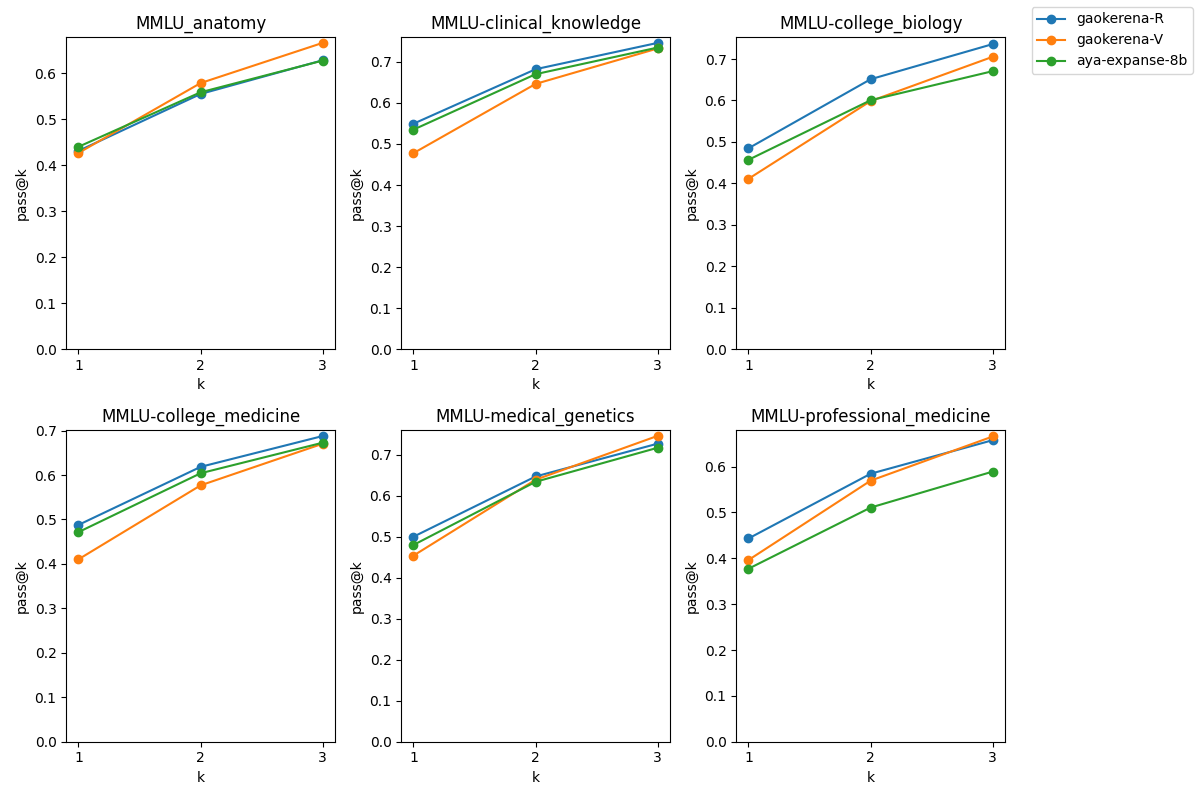
\includegraphics[width=1.0\linewidth]{fig8.png}
    \caption{Pass@k results on the Persian Translated Medical Portion of MMLU dataset}
    \label{fig8}
\end{figure}

\begin{figure}[h]
    \centering
    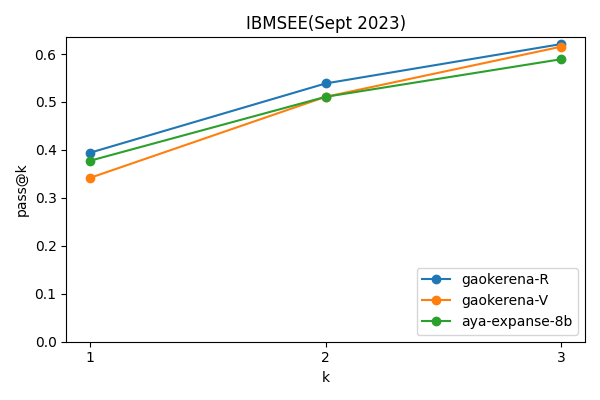
\includegraphics[width=0.8\linewidth]{fig9.png}
    \caption{Pass@k results on the IBMSEE Sept2023 dataset}
    \label{fig9}
\end{figure}

\subsection{Uncertainty Head Results}
\label{sec:uhead_results}
We now evaluate the claim-level uncertainty heads trained in Section~\ref{sec:uhead}. Following the protocol described there, each head is selected on the 92-response validation split using PR-AUC and then scored once on the 50-response test split, which is never seen during training or model selection. The task is binary classification at the level of an individual extracted claim: the head must decide whether a claim produced by the frozen backbone is factually supported or hallucinated. Table~\ref{tab:uhead_results} reports all metrics as percentages.

Two properties of the evaluation must be kept in mind when reading the numbers. First, the task is strongly imbalanced: only 20.95\% of the 1{,}951 claims in the Gaokerena-V test split and 17.46\% of the 1{,}687 claims in the Gaokerena-R split are hallucinated. A trivial classifier that flags nothing therefore achieves 79.05\% and 82.54\% accuracy respectively, so accuracy alone is close to uninformative here, and PR-AUC is the metric of record. Second, the expected PR-AUC of a random classifier equals the positive base rate, so the two heads must be judged against \emph{different} floors---0.2095 and 0.1746. Raw PR-AUC is consequently not directly comparable between them, and we report the ratio to each floor alongside it. Results are reported in Table~\ref{tab:uhead_results}.

The Gaokerena-V head reaches a PR-AUC of 0.4820, which is 2.30 times the 0.2095 random baseline, and a ROC-AUC of 0.7852 against a random baseline of 0.5. The head therefore extracts a substantial and genuine hallucination signal from the frozen backbone's attention maps and token probabilities alone, without retrieval, without reference text, and without repeated sampling. At its operating point it identifies 58.17\% of hallucinated claims (recall) with 44.85\% of its flags being correct (precision); the latter figure is more than twice the 20.95\% precision a random flag would achieve. For the intended use---surfacing claims that warrant human verification in a medical setting---this recall-favouring balance is the more useful trade-off, since the cost of an unreviewed hallucination exceeds the cost of an unnecessary review.

The training dynamics are also informative. Validation PR-AUC peaked at epoch 3 (0.4911) and did not improve thereafter, triggering early stopping at epoch 6 out of a configured maximum of 10. The head thus converges quickly, which is consistent with its small parameter count relative to the 8-billion-parameter frozen backbone. The close agreement between validation PR-AUC at the selected epoch (0.4911) and test PR-AUC (0.4820) indicates that model selection on the validation split did not overfit, and that the reported test figure is a fair estimate of generalisation.

The Gaokerena-R head, trained on the paired \texttt{LUH-Gaokerena-R} dataset under an identical configuration, reaches a PR-AUC of 0.4652 and a ROC-AUC of 0.7810. Its validation PR-AUC peaked at epoch 4 (0.4108), with early stopping at epoch 7. Read naively, its PR-AUC is 0.0168 below that of the Gaokerena-V head; but because its test split is less imbalanced, the correct comparison is against its own floor, and there the ordering reverses: 2.66 times random for Gaokerena-R against 2.30 times for Gaokerena-V.

The most informative comparison is ROC-AUC, which unlike PR-AUC is invariant to the positive base rate. The two heads are separated by 0.42 percentage points (0.7852 against 0.7810), which is negligible. Our reading is therefore that the hallucination signal is \emph{equally learnable} from both backbones: replacing the knowledge-oriented Gaokerena-V with the reasoning-oriented Gaokerena-R neither helps nor harms a claim-level uncertainty head. Given that the paired design holds the questions, the row indices, the annotation pipeline, and every hyperparameter fixed, this near-equality is attributable to the backbone substitution itself.

The remaining differences in Table~\ref{tab:uhead_results} are operating-point artifacts rather than differences in discriminative power, and should not be over-read. The Gaokerena-R head is markedly more recall-oriented, flagging 80.84\% of hallucinated claims at 29.52\% precision, where the Gaokerena-V head flags 58.17\% at 44.85\%. This follows from which epoch PR-AUC selection happened to choose: as the per-epoch validation traces show, both runs oscillate between high-precision and high-recall regimes across adjacent epochs, and the selected checkpoints landed on opposite sides of that trade-off. Accuracy and F1 inherit the same arbitrariness, which is a further reason to treat the threshold-free AUCs as primary. A deployment would in any case tune the decision threshold to the desired review budget rather than accept the checkpoint's default.

Two caveats bound how strongly these results should be read. Each test split contains only 50 responses, and although this yields 1{,}951 and 1{,}687 claims, the claims within a response are correlated, so the effective sample is considerably smaller than the claim count suggests. Differences of the magnitude seen here between the two heads are within that uncertainty. Relatedly, the Gaokerena-R head scores higher on test (0.4652) than on validation at its selected epoch (0.4108), whereas the Gaokerena-V head scores slightly lower on test than validation; with splits this small, such reversals are expected and neither should be interpreted as a systematic effect.

\begin{table}[ht]
\centering
\begin{tabular}{|l|c|c|}
\hline
\textbf{Metric} & \textbf{Gaokerena-V} & \textbf{Gaokerena-R} \\ \hline
Accuracy & \textbf{76.24} & 62.96 \\ \hline
Precision & \textbf{44.85} & 29.52 \\ \hline
Recall & 58.17 & \textbf{80.84} \\ \hline
F1 & \textbf{50.65} & 43.24 \\ \hline
ROC-AUC & \textbf{78.52} & 78.10 \\ \hline
PR-AUC & \textbf{48.20} & 46.52 \\ \hline
Random PR-AUC & & \\
(base rate) & 20.95 & 17.46 \\ \hline
PR-AUC / random & 2.30 & \textbf{2.66} \\ \hline
Test claims & 1{,}951 & 1{,}687 \\ \hline
Selected epoch & 3 & 4 \\ \hline
\end{tabular}
\caption{Claim-level uncertainty head performance on the held-out test split.}
\label{tab:uhead_results}
\end{table}


	\begin{thebibliography}{00}
		\bibitem{b1} 
		Ghassabi, Mehrdad, et al. "Leveraging online data to enhance medical knowledge in a small persian language model." 2025 32nd National and 10th International Iranian Conference on Biomedical Engineering (ICBME). IEEE, 2025.
                   \bibitem{b2}
                  Ghassabi, Mehrdad, et al. "Enhancing Reasoning Skills in Small Persian Medical Language Models Can Outperform Large-Scale Data Training." 2025 11th International Conference on Signal Processing and Intelligent Systems (ICSPIS). IEEE, 2025.
		\bibitem{b3} 
		Vaswani, Ashish, et al. "Attention is all you need." Advances in neural information processing systems 30 (2017).
                   \bibitem{b4}
                   Wu, Juncheng, et al. "Medreason: Eliciting factual medical reasoning steps in llms via knowledge graphs. ArXiv, abs/2504.00993, 2025."
                   \bibitem{b5}
                   Taghizadeh, Nasrin, et al. "SINA-BERT: a pre-trained language model for analysis of medical texts in Persian." arXiv preprint arXiv:2104.07613 (2021).
                   \bibitem{b6}
                   Kim, Hyunjae, et al. "Small language models learn enhanced reasoning skills from medical textbooks." arXiv preprint arXiv:2404.00376 (2024).
                   \bibitem{b7}
                   Wei, Jason, et al. "Chain-of-thought prompting elicits reasoning in large language models." Advances in neural information processing systems 35 (2022): 24824-24837.
                   \bibitem{b8}
                    Jiang, Shuyang, et al. "MedS3: Towards Medical Slow Thinking with Self-Evolved Soft Dual-sided Process Supervision." Proceedings of the AAAI Conference on Artificial Intelligence. Vol. 40. No. 37. 2026.
                   \bibitem{b9}
                  Vishwanath, Krithik, et al. "MedMobile: A mobile-sized language model with clinical capabilities." arXiv preprint arXiv:2410.09019 (2024).
                   \bibitem{b10}
                   Abdin, Marah, et al. "Phi-3 Technical Report: A Highly Capable Language Model Locally on Your Phone." arXiv, 30 Aug. 2024, arxiv.org/abs/2404.14219.
                   \bibitem{b11}
                   Dang, John, et al. "Aya expanse: Combining research breakthroughs for a new multilingual frontier." arXiv preprint arXiv:2412.04261 (2024).
                   \bibitem{b12}
                   Rostami, Pedram, Ali Salemi, and Mohammad Javad Dousti. "Persianmind: A cross-lingual persian-english large language model." arXiv preprint arXiv:2401.06466 (2024).
                   \bibitem{b13}
                   Touvron, Hugo, et al. "Llama 2: Open foundation and fine-tuned chat models." arXiv preprint arXiv:2307.09288 (2023).
                    \bibitem{b14}
		García-Ferrero, Iker, et al. "Medical mT5: an open-source multilingual text-to-text LLM for the medical domain." arXiv preprint arXiv:2404.07613 (2024).
                    \bibitem{b15}
		Liu, Yang, et al. "Datasets for large language models: A comprehensive survey." arXiv preprint arXiv:2402.18041 (2024).
                    \bibitem{b16}
                   Li, Yunxiang, et al. "Chatdoctor: A medical chat model fine-tuned on a large language model meta-ai (llama) using medical domain knowledge." Cureus 15.6 (2023).
                    \bibitem{b17}
		Yang, Songhua, et al. "Zhongjing: Enhancing the chinese medical capabilities of large language model through expert feedback and real-world multi-turn dialogue." Proceedings of the AAAI conference on artificial intelligence. Vol. 38. No. 17. 2024.
		\bibitem{b18}
		Bao, Zhijie, et al. "Disc-medllm: Bridging general large language models and real-world medical consultation." arXiv preprint arXiv:2308.14346 (2023).
		\bibitem{b19}
		Zhang, Hongbo, et al. "Huatuogpt, towards taming language model to be a doctor." arXiv preprint arXiv:2305.15075 (2023).
		\bibitem{b20}
		Wang, Xidong, et al. "Huatuo-26M, a Large-scale Chinese Medical QA Dataset." Findings of the Association for Computational Linguistics: NAACL 2025. 2025.
		\bibitem{b21}
		Zeng, Guangtao, et al. "MedDialog: Large-scale medical dialogue datasets." Proceedings of the 2020 conference on empirical methods in natural language processing (EMNLP). 2020.
		\bibitem{b22}
		Han, Tianyu, et al. "MedAlpaca--an open-source collection of medical conversational AI models and training data." arXiv preprint arXiv:2304.08247 (2023).
                   \bibitem{b23}
                   Manes, Itay, et al. "K-qa: A real-world medical q\&a benchmark." arXiv preprint arXiv:2401.14493 (2024).
                   \bibitem{b24}
                   Hendrycks, Dan, et al. "Measuring massive multitask language understanding." arXiv preprint arXiv:2009.03300 (2020).
                   \bibitem{b25}
                   Bi, Xiao, et al. "Deepseek llm: Scaling open-source language models with longtermism." arXiv preprint arXiv:2401.02954 (2024).
                    \bibitem{b26}
                   Pal, Ankit, Logesh Kumar Umapathi, and Malaikannan Sankarasubbu. "Medmcqa: A large-scale multi-subject multi-choice dataset for medical domain question answering." Conference on health, inference, and learning. PMLR, 2022.
                   \bibitem{b27}
                   xAI. "Grok 3 Beta — The Age of Reasoning Agents." xAI Blog, 17 Feb. 2025, x.ai/news/grok-3.
                   \bibitem{b28}
                   Achiam, Josh, et al. "Gpt-4 technical report." arXiv preprint arXiv:2303.08774 (2023).
                   \bibitem{b29}
                   Hu, Edward J., et al. "Lora: Low-rank adaptation of large language models." ICLR 1.2 (2022): 3.
                    \bibitem{b30}
                   Lee, Harrison, et al. "Rlaif vs. rlhf: Scaling reinforcement learning from human feedback with ai feedback." arXiv preprint arXiv:2309.00267 (2023).
                   \bibitem{b31}
                    Rafailov, Rafael, et al. "Direct preference optimization: Your language model is secretly a reward model." Advances in neural information processing systems 36 (2023): 53728-53741.
                   \bibitem{b32}
                    Guo, Daya, et al. "Deepseek-r1: Incentivizing reasoning capability in llms via reinforcement learning." arXiv preprint arXiv:2501.12948 (2025).
                    \bibitem{b33}
                    Shelmanov, Artem, et al. "Uncertainty quantification for large language models." Proceedings of the 63rd Annual Meeting of the Association for Computational Linguistics (Volume 5: Tutorial Abstracts). 2025.
                    \bibitem{b34}
                   Q. jiang, Albert et al. "Mistral7b" arXiv preprint arXiv:2310.06825 (2023).
                   \bibitem{b35}
                   Ahmadian, Arash, et al. "Mix data or merge models? optimizing for diverse multi-task learning." arXiv preprint arXiv:2410.10801 (2024).
                   \bibitem{b36}
                   DeepSeek-AI, Anyi Xu, et al. "Deepseek-v4: Towards highly efficient million-token context intelligence."
                    \bibitem{b37}
		Yang, An, et al. “Qwen2 Technical Report.” arXiv Preprint arXiv:2407.10671, 2024.
                   \bibitem{b38}
                   Wang, Xuezhi, et al. "Self-consistency improves chain of thought reasoning in language models." arXiv preprint arXiv:2203.11171 (2022).
                   \bibitem{b39}
                    Brown, Bradley, et al. "Large language monkeys: Scaling inference compute with repeated sampling." arXiv preprint arXiv:2407.21787 (2024).

                    

	\end{thebibliography}
	

\end{document}